\documentclass{standalone}
\usepackage{../../../../preamble_formulas}

\begin{document}
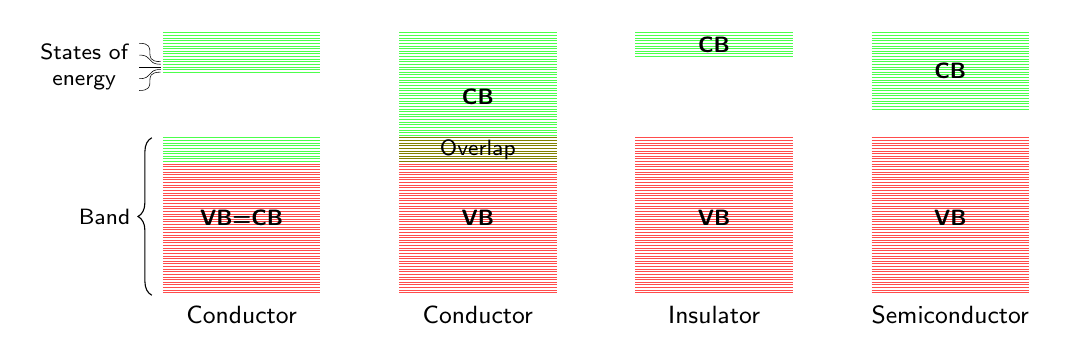
\begin{tikzpicture}
  \sffamily

  % Conductor
  \foreach \i in{1,...,50}{
      \draw[very thin, red!70] (0,\i/30) -- (2,\i/30);
    }
  \foreach \i in{51,...,60}{
      \draw[very thin, green!70] (0,\i/30) -- (2,\i/30);
    }
  \foreach \i in{85,...,100}{
      \draw[very thin, green!70] (0,\i/30) -- (2,\i/30);
    }
  \node[font=\small] at (1,-0.25){Conductor};
  \node[font=\footnotesize] at (1,0.983){\textbf{VB=CB}};

  % Conductor
  \foreach \i in{1,...,50}{
      \draw[very thin, red!70] (3,\i/30) -- (5,\i/30);
    }
  \foreach \i in{51,...,60}{% overlap
      \draw[very thin, green!50!red] (3,\i/30) -- (5,\i/30);
    }
  \foreach \i in{61,...,100}{
      \draw[very thin, green!70] (3,\i/30) -- (5,\i/30);
    }
  \node[font=\small] at (4,-0.25){Conductor};
  \node[font=\footnotesize] at (4,2.5167){\textbf{CB}};
  \node[font=\footnotesize] at (4,0.983){\textbf{VB}};
  \node[font=\footnotesize] at (4,1.85){Overlap};

  % Insulator
  \foreach \i in{1,...,60}{
      \draw[very thin, red!70] (6,\i/30) -- (8,\i/30);
    }
  \foreach \i in{91,...,100}{
      \draw[very thin, green!70] (6,\i/30) -- (8,\i/30);
    }
  \node[font=\small] at (7,-0.25){Insulator};
  \node[font=\footnotesize] at (7,3.1833){\textbf{CB}};
  \node[font=\footnotesize] at (7,0.983){\textbf{VB}};

  % Semiconductor
  \foreach \i in{1,...,60}{
      \draw[very thin, red!70] (9,\i/30) -- (11,\i/30);
    }
  \foreach \i in{71,...,100}{
      \draw[very thin, green!70] (9,\i/30) -- (11,\i/30);
    }
  \node[font=\small] at (10,-0.25){Semiconductor};
  \node[font=\footnotesize] at (10,2.85){\textbf{CB}};
  \node[font=\footnotesize] at (10,0.983){\textbf{VB}};

  \draw [decorate,decoration={brace,amplitude=5pt},xshift=-4pt,yshift=0pt]
  (0,0) -- (0,2) node [black,midway,xshift=-0.6cm] {\footnotesize Band};
  % \foreach \i in{85,...,88}{
  %     \draw[very thin] (-0.02,\i/30) -- (-0.5,2);
  %   }
  \draw[very thin] (-0.03, 89/30) .. controls (-0.3, 89/30) and (-0.03, 87/30+0.3) .. (-0.3, 87/30+0.3);
  \draw[very thin] (-0.03, 88/30) .. controls (-0.21,  88/30) and (-0.12,  87/30+0.15) .. (-0.3, 87/30+0.15);
  \draw[very thin] (-0.03, 87/30) -- (-0.3, 87/30);
  \draw[very thin] (-0.03, 86/30) .. controls (-0.21,  86/30) and (-0.12,  87/30-0.15) .. (-0.3, 87/30-0.15);
  \draw[very thin] (-0.03, 85/30) .. controls (-0.3,  85/30) and (-0.03,  87/30-0.3) .. (-0.3, 87/30-0.3);
  \node[font=\footnotesize, text width=1.2cm, align=center] at (-1,2.9){States of energy};
\end{tikzpicture}
\end{document}